\documentclass{beamer}
\usepackage{fontspec} 
\usepackage{soul}
\usepackage{tikz}
\usepackage{pgfplots}
\newcommand{\barplot}[4]{%
  \begin{tikzpicture}
    \begin{axis}[
	xlabel={#1},  
	ylabel={#2}, 
	axis lines*=left, 
        width  = \textwidth,
	height = .3\textheight,
    	nodes near coords, 
	xtick=data,
	x tick label style={},  
	ymin=0,
	symbolic x coords={#3},
	]
	\addplot+[ybar,lsRichGreen!80!black,fill=lsRichGreen] plot coordinates {
	    #4
	}; 
    \end{axis} 
  \end{tikzpicture} 
}

\useoutertheme{lsp}

\usepackage{lsptitle}

\def\two@digits#1{\ifnum#1<10 0\fi\number#1}
\def\mytoday{\two@digits{\number\day}.\two@digits{\number\month}.\number\year}


\usepackage{xspace,multicol}
\newcommand{\latex}{\LaTeX\xspace}
\usepackage{tikz}


\newcounter{lastpagemainpart}
\footnotesep0pt
\renewcommand{\footnoterule}{}
\usefootnotetemplate{
  \noindent
  \insertfootnotemark\insertfootnotetext}

\let\beamerfn=\footnote
\renewcommand{\footnote}[1]{%
\let\oldfnsize=\footnotesize%
\let\footnotesize=\tiny%
\beamerfn<\thebeamerpauses->{#1}%
\let\footnotesize=\oldfnsize}


\date{25.2.2019}

\usepackage{eurosym}  
 
\renewcommand{\centerline}[1]{\hfill#1\hfill\hfill\mbox{}}


\title{\mbox{Establishing a non-APC/BPC} publishing initiative}
% \institute{FU Berlin}
\author[LangSci]{Sebastian Nordhoff}



\begin{document}
\lspbeamertitle


\section{Introduction}
\frame{
\frametitle{Language Science Press}
\begin{itemize}
 \item since 2014
 \item monographs and edited volumes in linguistics
 \item only OA
 \item 85 books published as of today 
 \item target: 30 books/year
 \item 23 series; 1003 supporters; 350 community proofreaders
\end{itemize}
}

\frame{
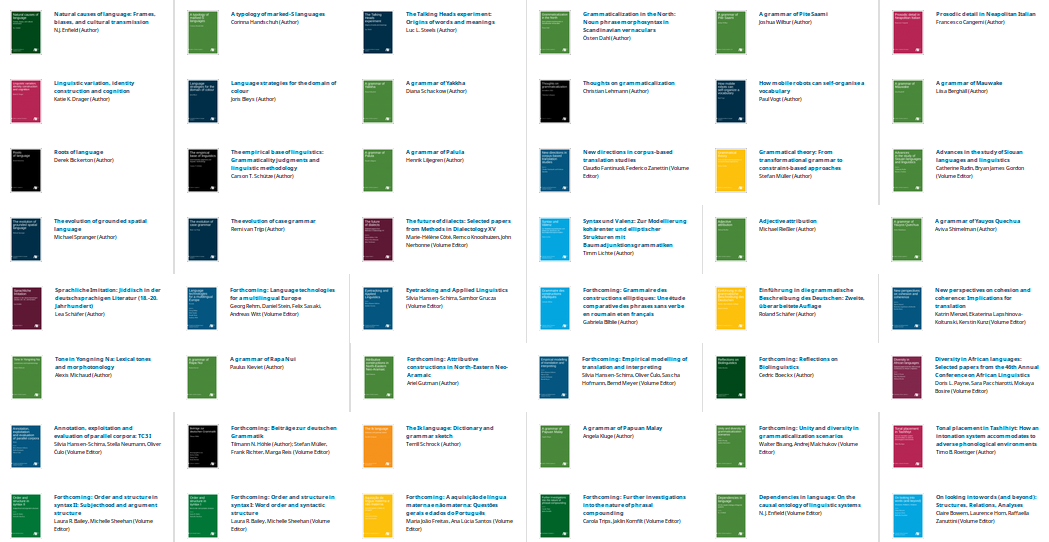
\includegraphics[width=\textwidth]{catalog.png}
}

\section{Business model}
\frame{
\frametitle{OpenAire non-BPC²}
 \textit{Full disclosure:  replicable strategies for book
publications supplemented with empirical data}\\

\includegraphics[width=.35\textwidth]{businessmodel.png}\hfill
\includegraphics[width=.35\textwidth]{cookbook.png}\hfill
~

\url{langsci-press.org/opendata}
}
% 
% \frame{
% \frametitle{Starting your own publishing project, Lesson I}
% ~
% \pause
% 
\includegraphics[height=\textheight]{whocares.jpg}
% }

\frame{
\frametitle{Who cares?}
\begin{tabular}{ll}
 readers & \\[1em]
 authors & \\[1em]
 institutions & \\[1em]
 society at large & \\
\end{tabular}
}

\frame{
\frametitle{Designing revenue streams}
\begin{tabular}{l@{~${\Longleftarrow}$~}l}
 readers & \fbox{\vphantom{fj}\st{subscription}} \fbox{\vphantom{fj}donations} \fbox{\vphantom{fj}membership}\\[1em]
 authors & \fbox{\vphantom{fj}BPCs} \fbox{\vphantom{fj}membership}\\[1em]
 institutions & \fbox{\vphantom{fj}institutional membership}\\[1em]
 society at large & \fbox{\vphantom{fj}funder-based platforms}\\
\end{tabular}
}


\frame{
\frametitle{Business model:\newline 
estimations \& projections} 
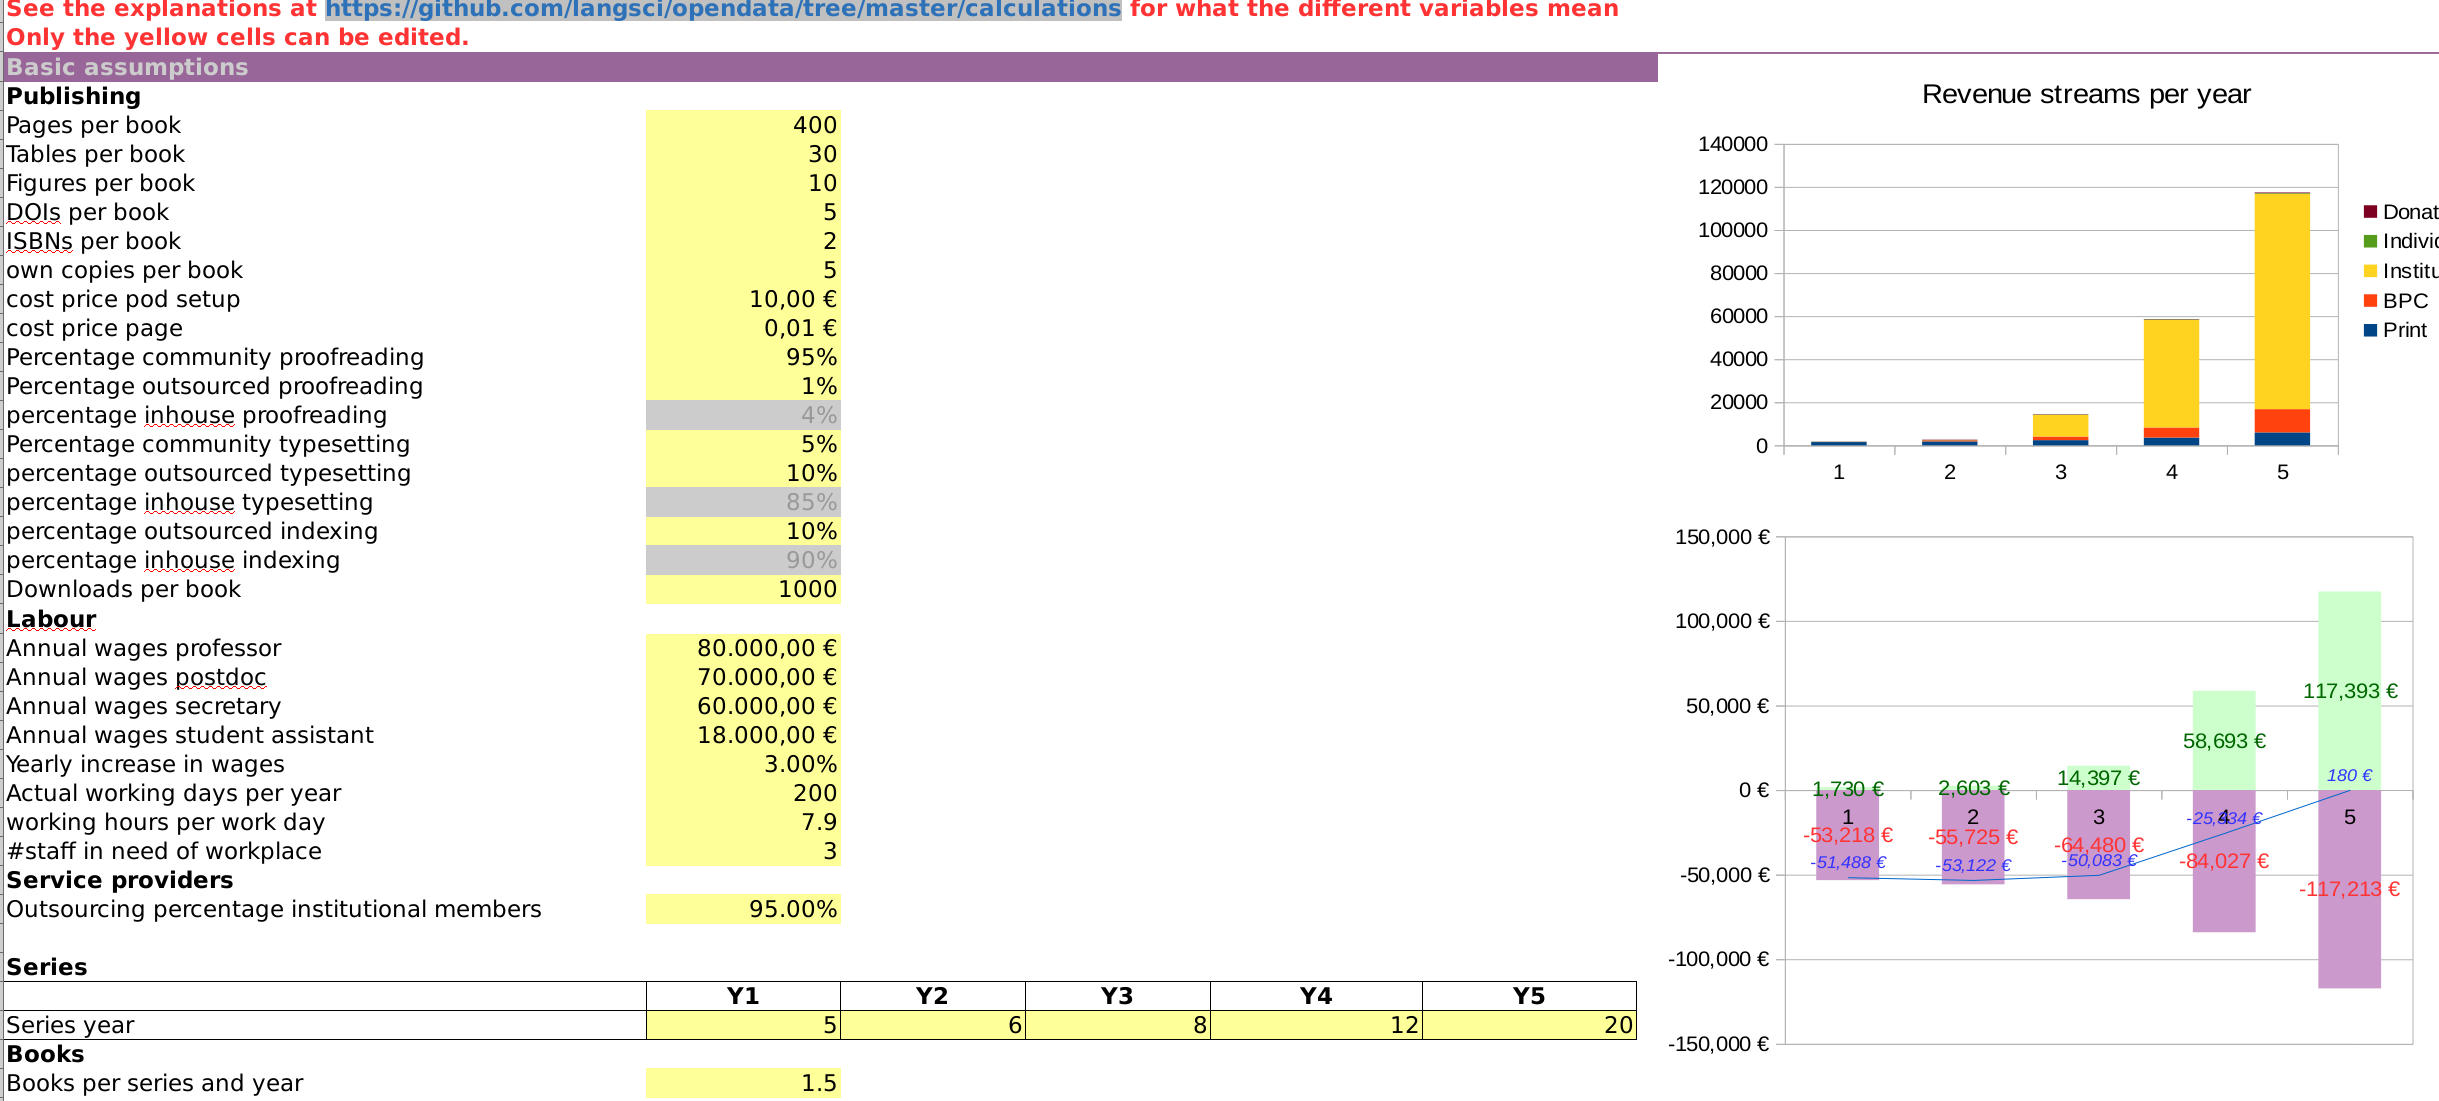
\includegraphics[width=\textwidth]{spreadsheet.png}
}


\frame{
\frametitle{Business model: projections}
  \begin{tikzpicture}
    \begin{axis}[
      scaled y ticks = false,
	y tick label style={/pgf/number format/fixed,
	/pgf/number format/1000 sep = \thinspace % Optional if you want to replace comma as the 1000 separator 
	},    
	xlabel={Revenue stream},  
	ylabel={EUR}, 
	axis lines*=left, 
        width  = \textwidth,
	height = \textheight,
    	nodes near coords, 
	xtick=data,
	x tick label style={},  
	ymin=0,
	symbolic x coords={individual m, donations, print margin, BPCs, institutional m},
	]
	\addplot+[ybar,lsRichGreen!80!black,fill=lsRichGreen] plot coordinates {
	  (individual m, 13200)
	  (donations, 9600)
	  (print margin, 24000)
	  (BPCs, 25200)
	  (institutional m, 56000)
	}; 
    \end{axis} 
  \end{tikzpicture} 
}

\frame{
\frametitle{Bureaucracy magic}

\includegraphics[width=\textwidth]{bureaucracymagic.png}
}


\frame{
\frametitle{Business model: Evaluation}
  \begin{tikzpicture}
    \begin{axis}[
    scaled y ticks = false,
      y tick label style={/pgf/number format/fixed,
      /pgf/number format/1000 sep = \thinspace % Optional if you want to replace comma as the 1000 separator 
      },
	xlabel={Revenue stream},  
	ylabel={EUR}, 
	axis lines*=left, 
        width  = \textwidth,
	height = \textheight,
    	nodes near coords, 
	xtick=data,
	x tick label style={},  
	ymin=0,
	ybar,
	symbolic x coords={individual m, donations, print margin, BPCs, institutional m},
	]
	\addplot[ybar,lsRichGreen!80!black,fill=lsRichGreen] plot coordinates {
	  (individual m, 13200)
	  (donations, 9600)
	  (print margin, 24000)
	  (BPCs, 25200)
	  (institutional m, 56000)
	}; 
	\addplot[ybar,lsDarkBlue!60!black,fill=lsDarkBlue!60!black] plot coordinates {
	  (individual m, 120)
	  (donations, 3000)
	  (print margin, 6000)
	  (BPCs, 2500)
	  (institutional m, 0)
	}; 
    \end{axis} 
  \end{tikzpicture} 
}

\section{Evaluation}
\frame{
\frametitle{Business model: Evaluation}
  \begin{tikzpicture}
    \begin{axis}[
    scaled y ticks = false,
      y tick label style={/pgf/number format/fixed,
      /pgf/number format/1000 sep = \thinspace % Optional if you want to replace comma as the 1000 separator 
      },
	scaled y ticks=false
	tick label style={/pgf/number format/fixed}
	xlabel={Revenue stream},  
	ylabel={EUR}, 
	axis lines*=left, 
        width  = \textwidth,
	height = \textheight,
    	nodes near coords, 
	xtick=data,
	x tick label style={},  
	ymin=0,
	ybar,
	symbolic x coords={individual m, donations, print margin, BPCs, institutional m},
	]
	\addplot+[ybar,lsRichGreen!80!black,fill=lsRichGreen] plot coordinates {
	  (individual m, 13200)
	  (donations, 9600)
	  (print margin, 24000)
	  (BPCs, 25200)
	  (institutional m, 56000)
	}; 
	\addplot+[ybar,lsDarkBlue!60!black,fill=lsDarkBlue!60!black] plot coordinates {
	  (individual m, 120)
	  (donations, 3000)
	  (print margin, 6000)
	  (BPCs, 2500)
	  (institutional m, 85000)
	}; 
    \end{axis} 
  \end{tikzpicture} 
}



\frame{
\frametitle{Sharing is caring: GitHub} 
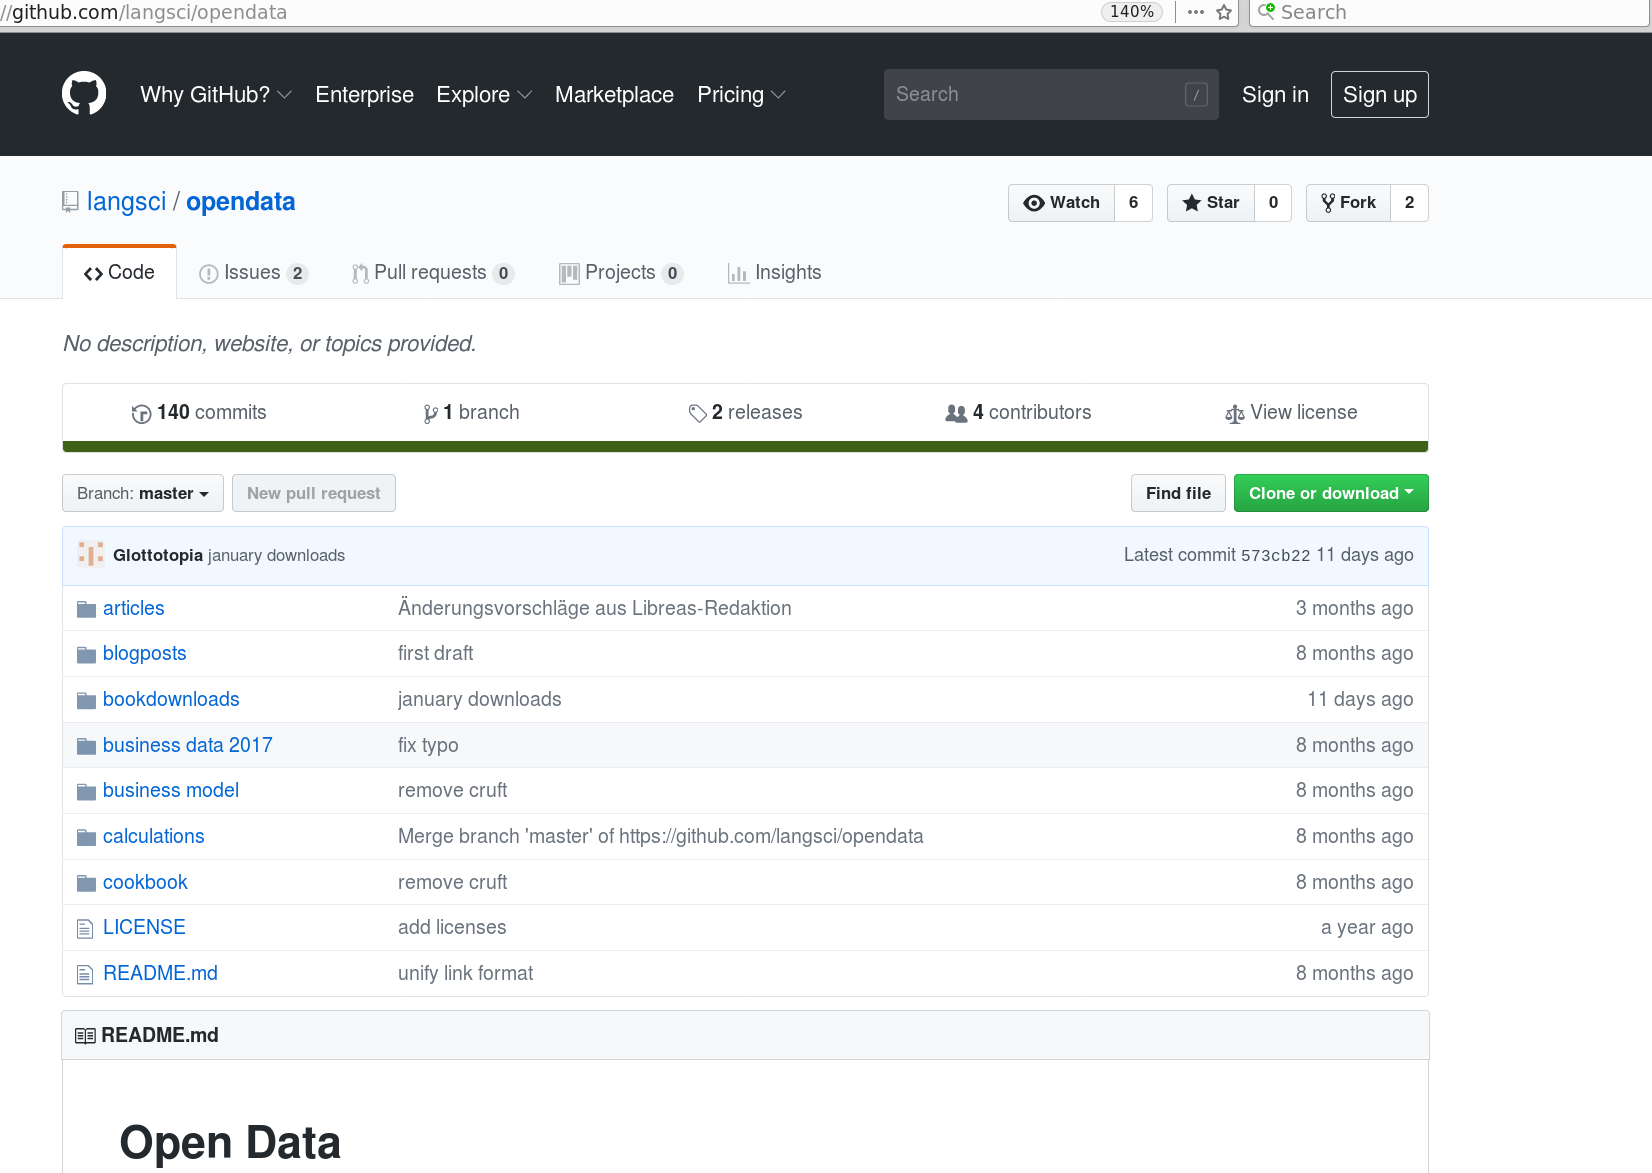
\includegraphics[width=\textwidth]{github.png}
}

\frame{
\frametitle{Sharing is caring:\newline spreadsheet} 
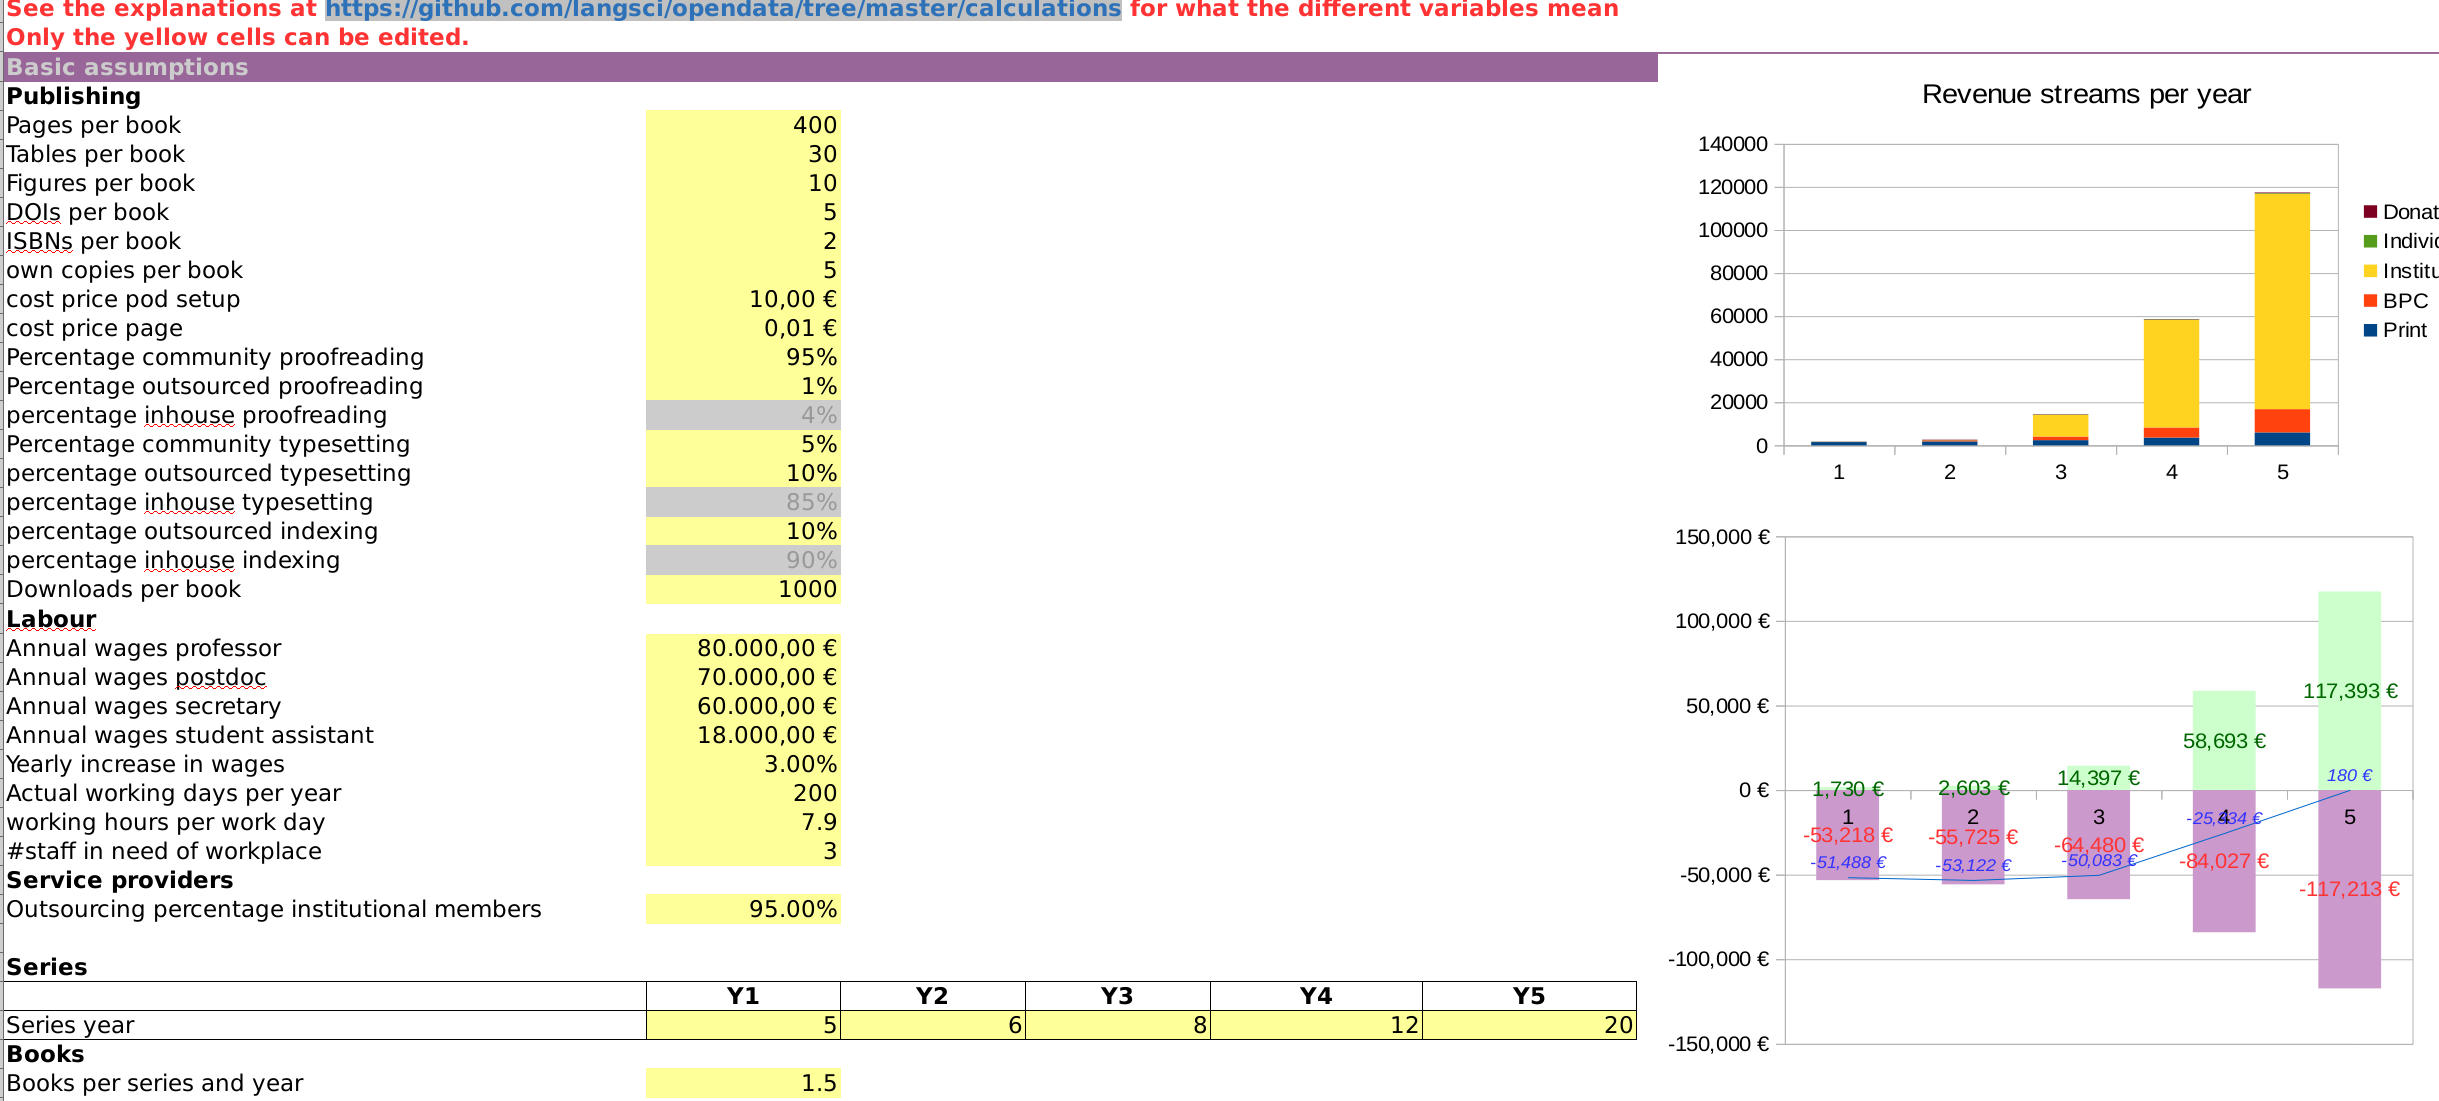
\includegraphics[width=\textwidth]{spreadsheet.png}
}



\frame{
\frametitle{But what if this does not work for me?}
\begin{itemize}
 \item work on alternatives
 \item specify the alternatives 
 \item evaluate the alternatives 
 \item share the alternatives
 \begin{itemize}
  \item best practices, lessons learned
 \end{itemize}
\end{itemize}
}

\frame{

\includegraphics[width=.4\textwidth]{businessmodel.png}\hfill
\includegraphics[width=.4\textwidth]{cookbook.png}\hfill
~
\url{langsci-press.org/opendata}
}

\frame{
\frametitle{Thank you}
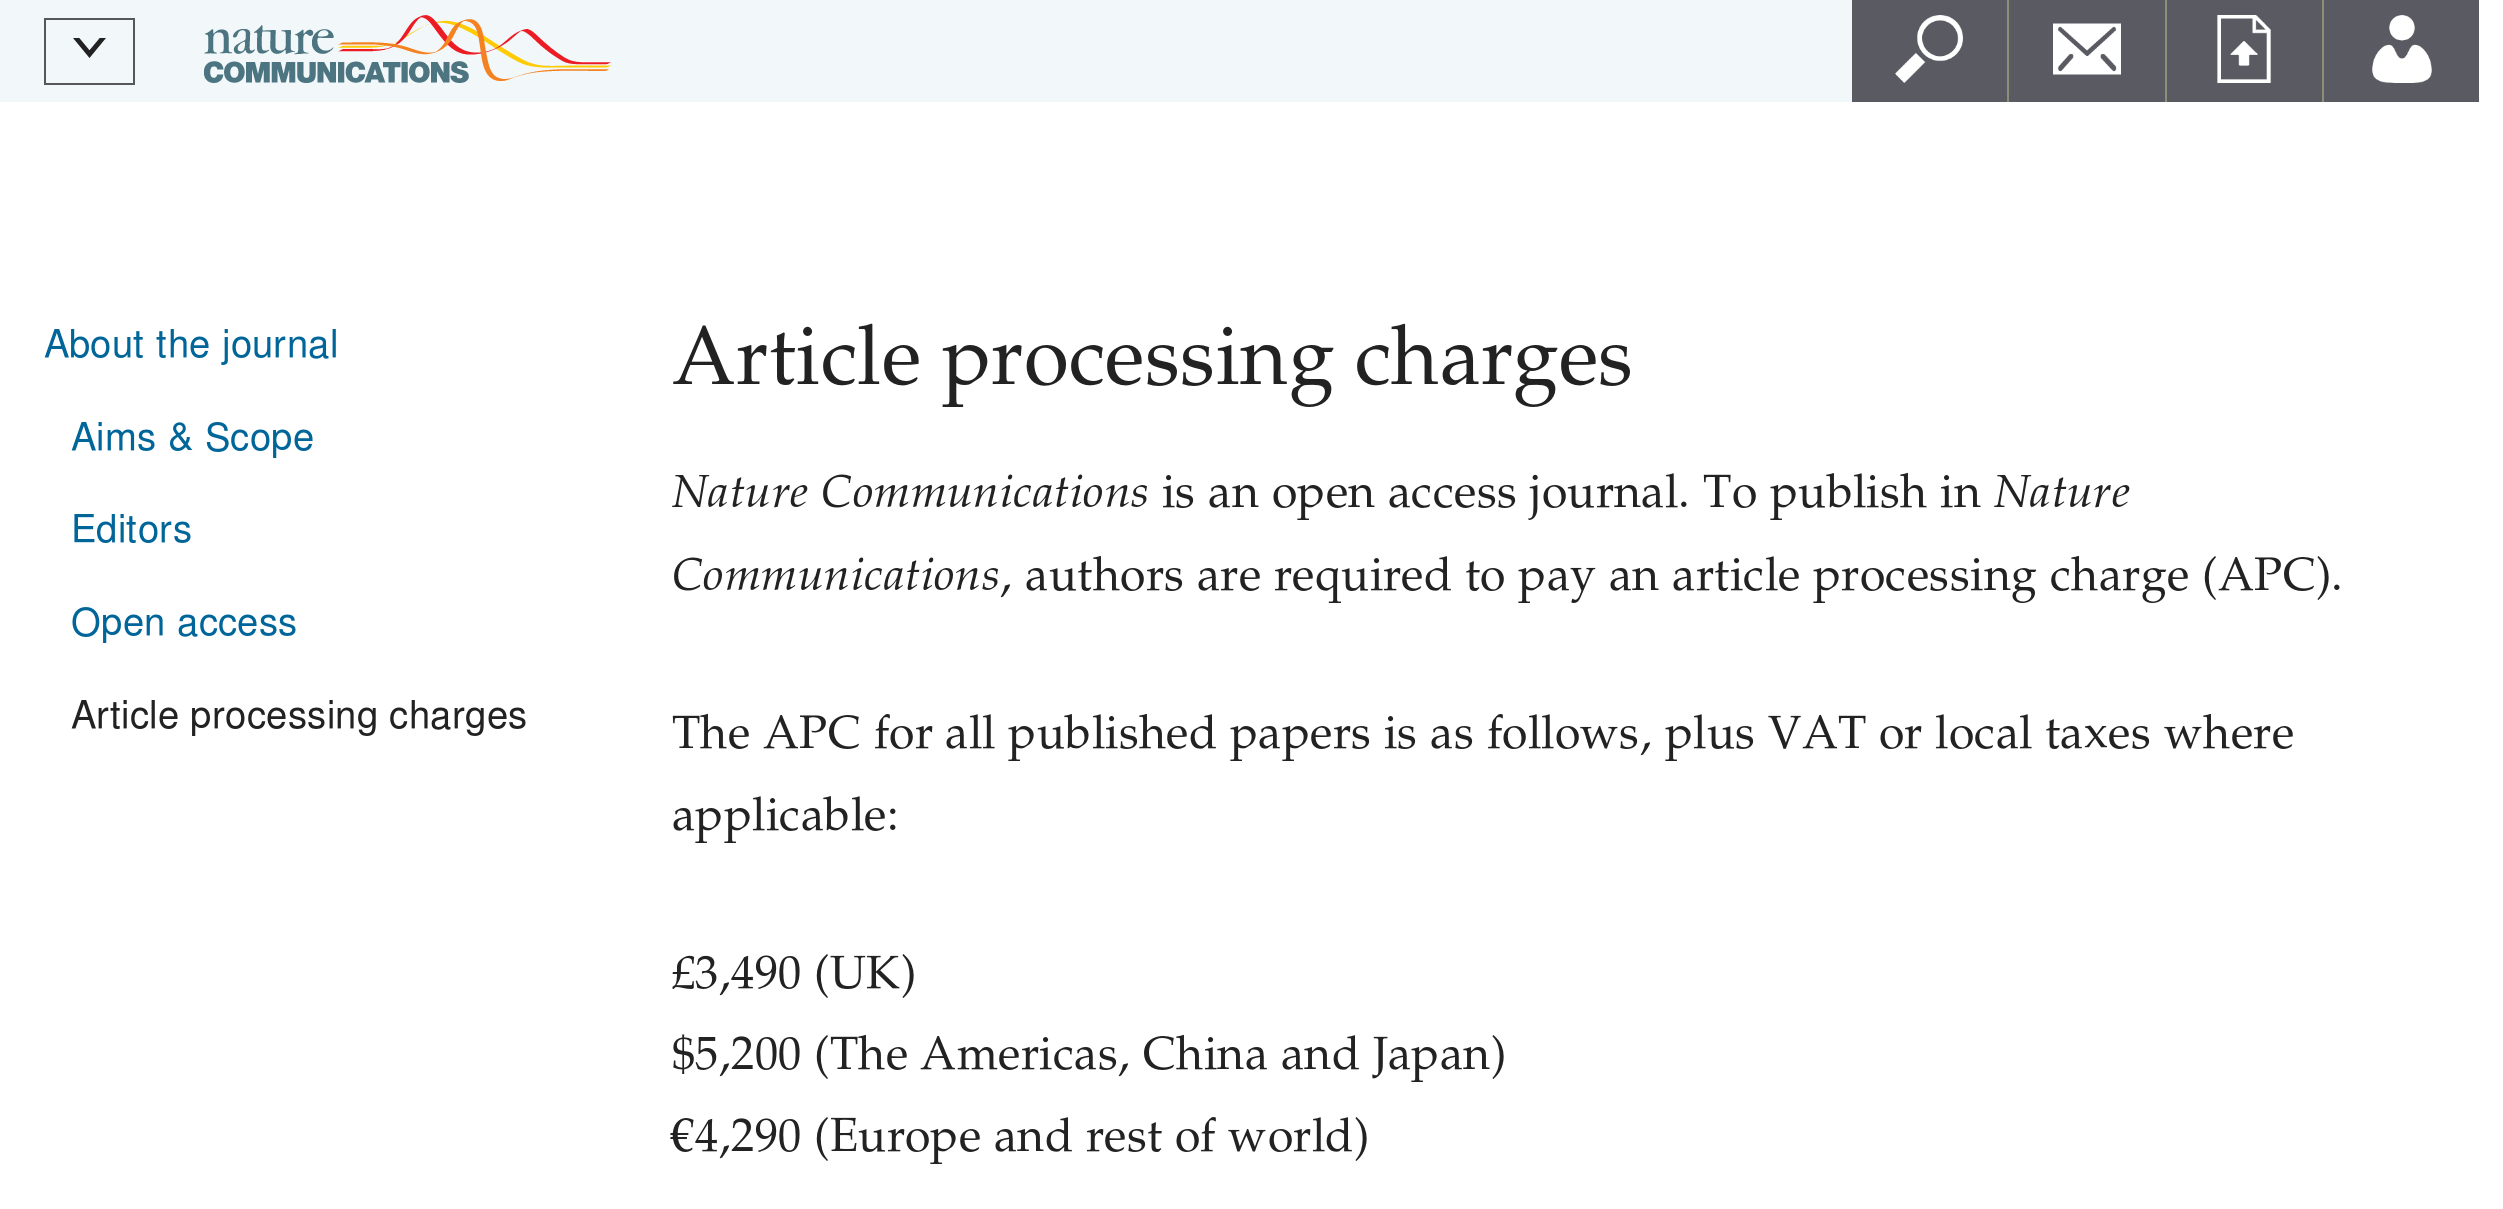
\includegraphics[width=\textwidth]{nature.png}
}

%\setcounter{framenumber}{\thelastpagemainpart}
\end{document}